\chapter{Tecnologie Abilitanti}
In questo capitolo verranno descritti gli strumenti e le tecnologie che sono stati utilizzati per la realizzazione dei requisiti software illustrati nel \textbf{Cap.2}.
\section{Realtà Virtuale}
La Realtà Virtuale\cite{VRRe} è un ambiente esclusivamente digitale creato da uno o più computer che simula la realtà effettiva e la ricrea in modo non tangibile e che viene visualizzato dall'utente tramite l'utilizzo di strumenti particolari, detti \textit{VR Headset}.
\\L'obiettivo principale di questa tecnologia è quello di ricreare un ambiente che stimoli il più possibile i 5 sensi, in modo da rendere il tutto molto più realistico.
\\L'architettura necessaria per poter usufruire in maniera completa della Realtà Virtuale è composta da:
\begin{itemize}
    \item Visori che abbiano determinate caratteristiche quali ad esempio un campo visivo dai 100 ai 110 gradi, un \textit{frame} rate (frequenza di immagini proiettate al secondo) compreso tra un minimo di almeno 60fps ed un massimo di 120fps per evitare una visione a scatti fastidiosa agli occhi
    \item Un giroscopio che consenta, insieme ad un accelerometro ed ad un magnetometro, il cosiddetto \textit{Head Tracking}, ovvero lo spostamento dell'immagine seguendo esattamente i movimenti del capo lungo i quattro punti cardinali e con tempi di risposta dai cinquanta millisecondi ai trenta millisecondi. 
    \\Tutto questo è sviluppato volutamente per far si che l'utente possa interagire e “vivere” all'interno della Realtà Virtuale. 
    \item La presenza all'interno del visore di un sistema audio professionale multicanale che offra la sensazione di suoni che provengono da tutte le direzioni e che consentano il cosiddetto effetto doppler (con l'aumentare del suono in avvicinamento ed il diminuire in allontanamento), sia da un sofisticato sistema di puntamento ad infrarossi che consente di leggere il movimento oculare (il cosiddetto \textit{eye tracking}) rendendo ancora più realistica l'immersione nell'ambiente virtuale mediante la creazione della profondità di campo.
\end{itemize} 
Nell'introduzione è stata illustrata l'utilità della Realtà Virtuale in ambito didattico, ma può essere impiegata in molteplici campi, come ad esempio nella medicina.
\\Nel campo medico la Realtà Virtuale sta diventando uno strumento non soltanto formativo, ma anche terapeutico ed operativo, con l'epilogo più famoso ad aprile di un anno fa al Royal London Hospital dove si è svolta in collegamento con l'India la prima operazione chirurgica della storia in realtà virtuale trasmessa in tempo reale.
\subsection{Headset}
\begin{figure}[H]
    \centering
    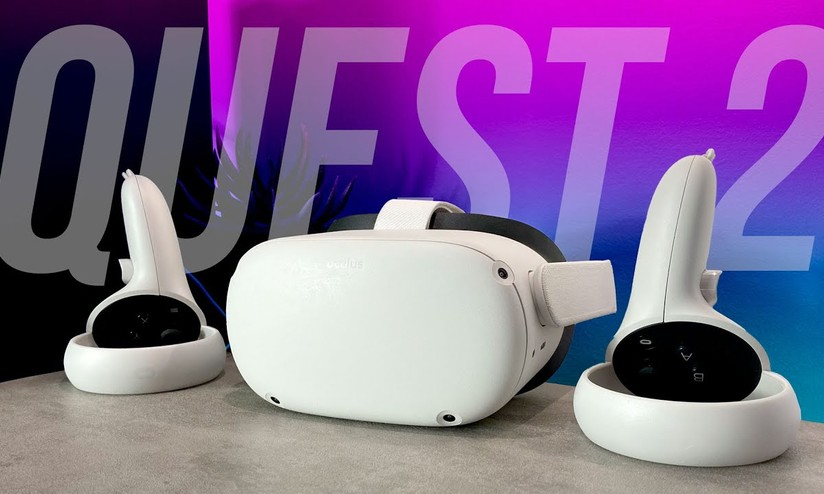
\includegraphics[scale = 0.5]{Immagini/Oculus-Quest-2.jpg}
    \caption{Oculus Quest 2 con i relativi controller}
    \label{fig:my_label}
\end{figure}
Un \textit{Virtual Reality Headset}\cite{Vrheadset}, o \textit{VR Headset}, è un dispositivo elettronico, detto visore, che permette la visone di applicazioni sviluppate per la Realtà Virtuale.\\Esistono due categorie di \textit{VR Headset}, quelli che necessitano di un collegamento ad un dispositivo Desktop e i dispositivi portatili con hardware dedicato.\\I primi sono i più indicati per lo sviluppo di ambienti in Realtà Virtuale sofisticati, visto che un PC è dotato di una potenza di calcolo mediamente superiore a quella di un dispositivo con hardware dedicato, ma di fatto ciò che l'utente vede è un semplice \gls{render} in tempo reale del mondo virtuale.\\I \textit{VR Headset} portatili con hardware integrato, o \textit{standalone} non offrono una resa grafica alla pari dei visori descritti precedentemente, ma permettono comunque di immergere l'utente in un'ambientazione verosimile, garantendo il vantaggio della portabilità.
\\Il prototipo sviluppato è stato pensato per essere utilizzabile sul modello di visore rappresentato nella \textbf{Figura 3.1}.
\\L'Oculus Quest 2 è un modello di visore \textit{standalone}, con esso è possibile non solo giocare ai giochi appositamente pensati per la Realtà Virtuale, ma anche guardare film come se si fosse al cinema, crearsi la propria configurazione multi-monitor per lavorare, visualizzare foto e video a 360 gradi, e fare tutto quello che ci viene in mente sempre immersi in un mondo virtuale.
\\Il visore si può configurare attraverso \textit{l'app Oculus}, scaricabile nel proprio \textit{smartphone}, e, una volta indossato, ci ritroveremo subito all'interno della \textit{home}, dalla quale potremo avviare tutte le \textit{app} e i giochi in nostro possesso. 
\\Nel mondo virtuale si può interagire con i \textit{controller} \textit{Oculus Touch}, le funzionalità pensate per gli utenti in questo prototipo si basano, perciò, sulle specifiche tecniche di questi \textit{controller}.
\section{Unity}
\begin{figure}[H]
    \centering
    
\includegraphics[scale = 0.2]{Immagini/ogimg.jpg}
    \caption{Logo di Unity}
    \label{fig:my_label}
\end{figure} 
\textbf{\textit{Unity}}\cite{unity} è un motore grafico per lo sviluppo di applicazioni 3D e 2D, anche in Realtà Virtuale, nato nel 2005.\\La progettazione di applicazioni è basata sul linguaggio di programmazione C\#(\textit{C sharp}), i cui \textit{\gls{script}} vengono gestiti tramite il software Microsoft Visual Studio.\\L'Editor di \textit{Unity} è supportato da Windows, MacOS e Linux, inoltre le applicazioni che si possono sviluppare sono supportate da piattaforme di vario tipo per esempio:
\begin{itemize}
    \item Mobili: IOS, Android;
    \item Desktop: Windows, MacOS, Linux;
    \item Web: WEBGL;
    \item Console: XBOX, Playstation(PS4, PS5), Nintendo Switch;
    \item Virtual Reality/Extended Reality: Oculus, PlayStation VR, Google's ARCore, Apple's ARKit, Windows Mixed Reality, Google Cardboard.
\end{itemize}
\subsection{Interfaccia Utente}
\begin{figure}[H]
    \centering
    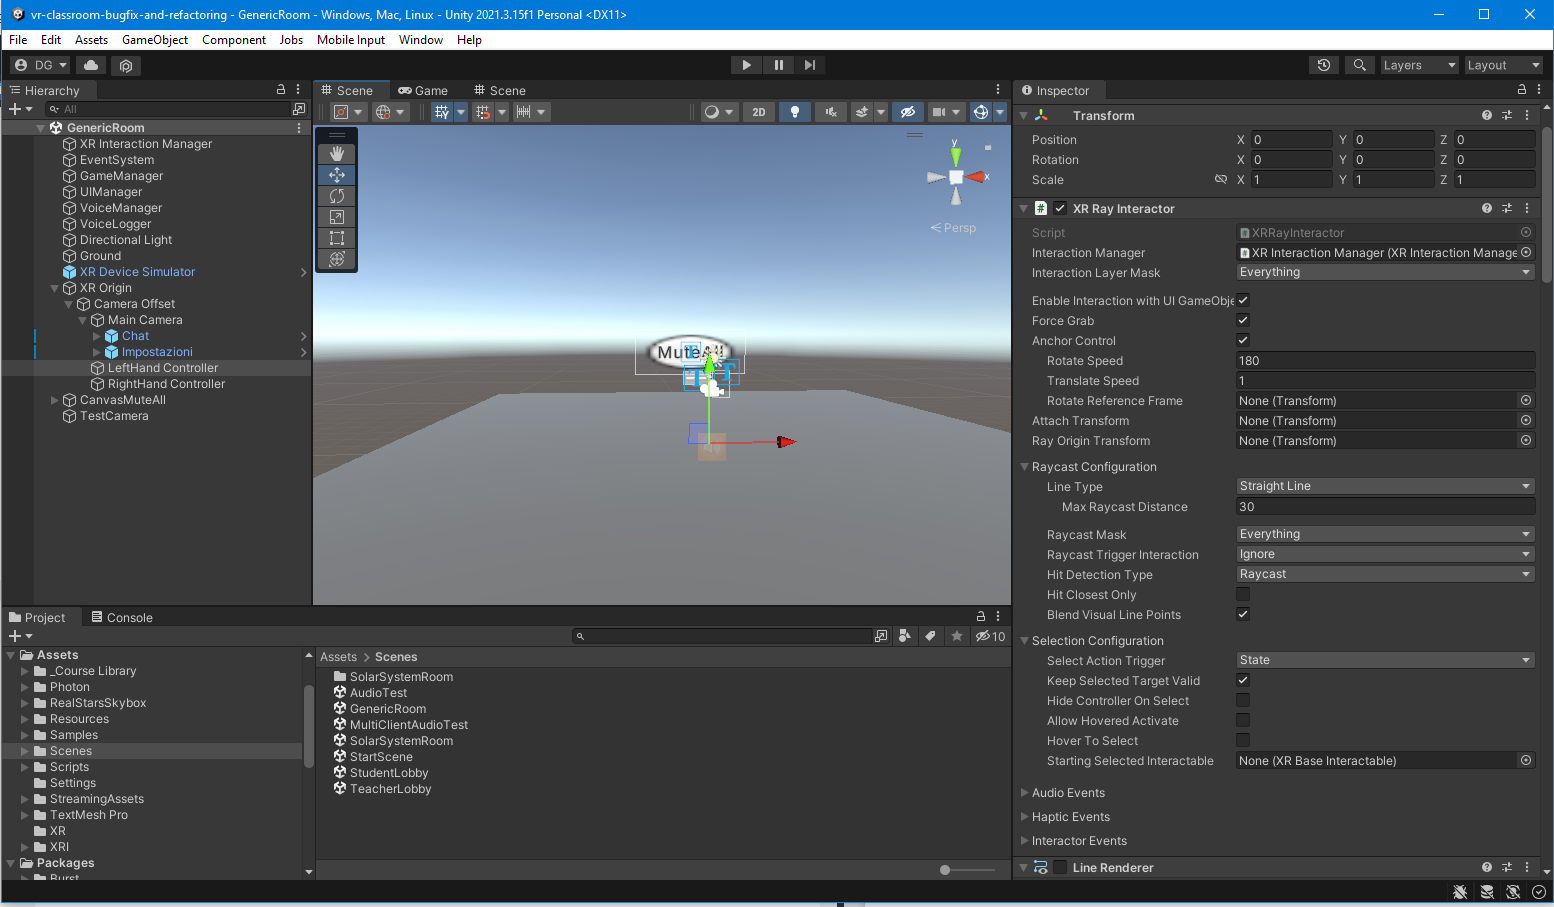
\includegraphics[scale = 0.35]{Immagini/UnityInteface.jpg}
    \caption{Interfaccia utente di Unity 2021.3.15f1}
    \label{fig:my_label}
\end{figure}
L'interfaccia utente\cite{unityMain} di \textit{Unity}, detta anche Unity Editor, è composta da 5 sezioni principali: Hierarchy, Game and Scene, Inspector, Project e Console.
\subsubsection{Hierarchy}
\begin{figure}[H]
    \centering
    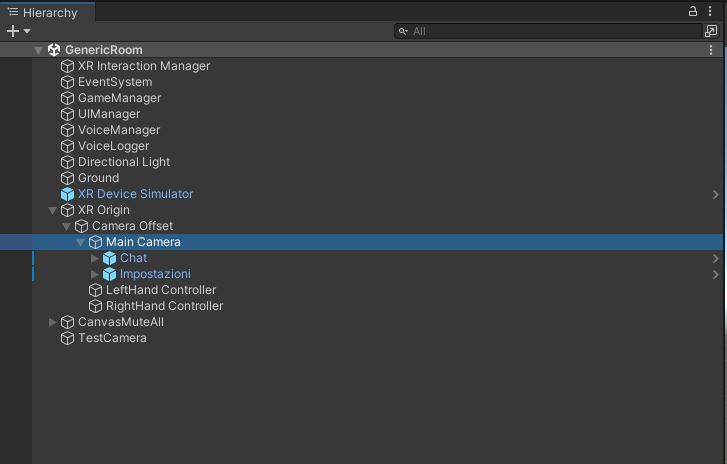
\includegraphics[width=12cm, height=9cm]{Immagini/Hierarchy.jpg}
    \caption{Hierarchy Panel di Unity Editor}
    \label{fig:my_label}
\end{figure}
La Hierarchy\cite{unityhierarchy} è la sezione dell'Editor in cui sono elencati tutti gli oggetti della scena e la relazione che c'è tra essi.\\La relazione tra oggetti è denominata gerarchia, o parentela, ovvero un oggetto può essere un `genitore` o `figlio` di un altro oggetto.\\È lo stesso tipo di relazione si può trovare tra cartelle nel \gls{File System} di un sistema operativo.\\L'oggetto principale, il genitore, trasmette le proprie componenti e proprietà agli oggetti figli, quindi ogni modifica effettuata sull'oggetto genitore verrà applicata anche all'oggetto figlio.\\La relazione di parentela può anche essere presente su più livelli, ossia un oggetto figlio può avere un oggetto figlio e così via.
\subsubsection{Game and Scene}
La Scena\cite{unityScene} è la sezione dell'Editor che rappresenta l'ambiente applicativo vero e proprio, in essa, infatti, sono visibili gli oggetti, detti \textit{GameObject}, che sono stati creati dal programmatore.\\Nella Scena, inoltre, si ha una visione interattiva dell'ambiente applicativo, ovvero è possibile posizionare, selezionare e manipolare gli oggetti.
\\Gli oggetti di scena possono essere di vario tipo per esempio: modelli 3D come cubi e sfere, modelli dotati di \textit{texture}, \textit{controller} per il giocatore, luci per l'ambientazione e una telecamera per rendere visibili tutti gli oggetti della scena, oltre alla scena stessa, nell'applicazione finale.
\\Dalla Scena si può entrare nella Game Mode\cite{unityGame}, quella sezione dell'Editor in cui è possibile testare ciò che si è creato nella Scena, come ad esempio i movimenti del giocatore e dei vari oggetti implementati nella Hierarchy.
\begin{figure}[H]
    \centering
    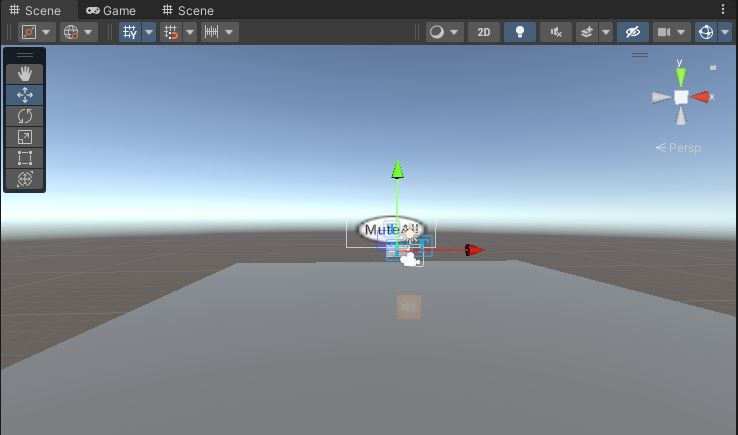
\includegraphics[scale = 0.6]{Immagini/Cattura.jpg}
    \caption{Game and Scene Panel di Unity Editor}
    \label{fig:my_label}
\end{figure}
\subsubsection{Inspector}
L'Inspector\cite{unityInspector} è la sezione dell'Editor dedicata alla gestione delle componenti degli oggetti \textit{Unity}, che possono essere di vario tipo, per esempio: script C\#, Transform, Text, Audio, Video ecc...
\\Sono le componenti dell'oggetto che determinano le funzionalità che ha all'interno della scena, per cui è essenziale applicare le componenti giuste agli oggetti per potergli permettere di compiere le azioni desiderate.
\\Ogni componente possiede dei parametri, che variano a seconda del tipo di componente, che posso essere modificati con mouse e tastiera tramite l'interfaccia utente.
\vspace*{0.5cm}
\begin{figure}[H]
    \centering
    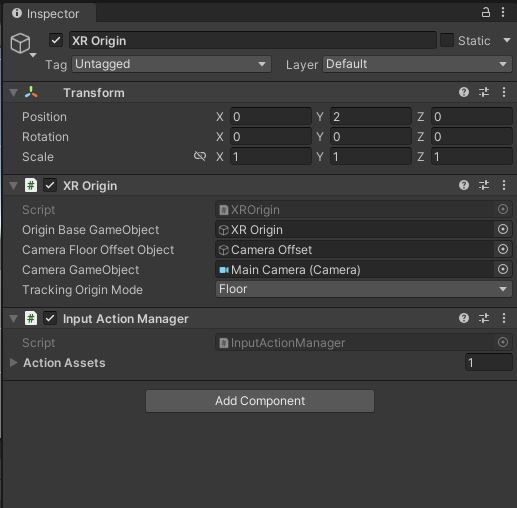
\includegraphics[scale = 1]{Immagini/Inspector.jpg}
    \caption{Inspector Panel di Unity Editor}
    \label{fig:my_label}
\end{figure}
\hspace{-0.6cm}È questo uno dei vantaggi che si ha nello sviluppo di applicazioni con \textit{Unity}, ovvero avere un'interfaccia interattiva nella quale si possono effettuare modifiche su oggetti e componenti che hanno effetto immediato sulla Scena.
\vspace{-2cm}
\subsubsection{Project}
Project\cite{unityProject} è la sezione dell'Editor che mostra la cartella `Assets` del progetto creato, che contiene tutti gli elementi che possono essere utilizzati all'interno del progetto.
\\Oltre agli elementi che si possono creare con \textit{Unity}, è possibile creare e importare elementi dell'Assets dall'esterno, come per esempio modelli 3D, file Audio, file Video, immagini o qualsiasi altro file compatibile con \textit{Unity}.
\vspace{1cm}
\begin{figure}[H]
    \centering
    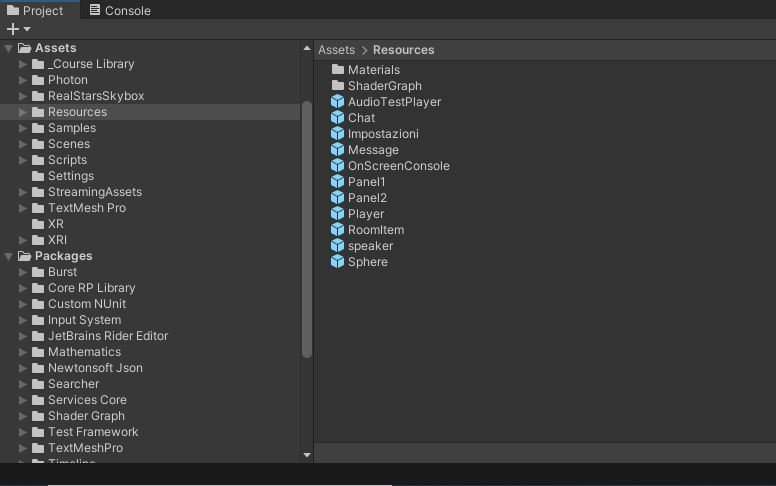
\includegraphics[scale = 0.7]{Immagini/Project.jpg}
    \caption{Project Panel di Unity Editor}
    \label{fig:my_label}
\end{figure}
\subsubsection{Console}
La Console\cite{unityconsole} è la sezione dell'Editor in cui si possono trovare i messaggi di errore, con il simbolo rosso, messaggi di avvertimento (\textit{warning}) e altri messaggi generati da \textit{Unity}.
\begin{figure}[H]
    \centering
    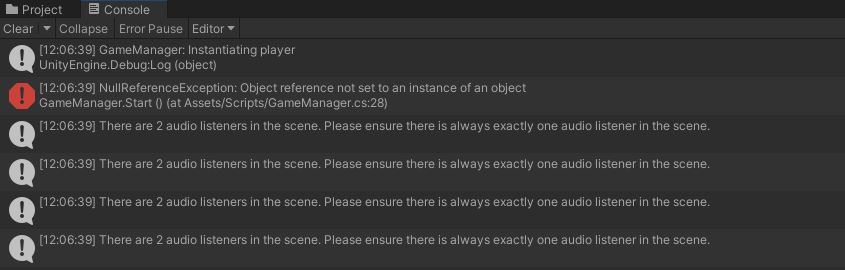
\includegraphics[scale = 0.75]{Immagini/Console.jpg}
    \caption{Console Panel di Unity Editor}
    \label{fig:my_label}
\end{figure}
\hspace{-0.6cm}Si possono anche generare manualmente dei messaggi sulla Console utilizzando i comandi \\\textit{\underline{Debug.Log}}, \textit{\underline{Debug.LogWarning}}, \textit{\underline{Debug.LogError}}.
\section{C\#}
Il C\#\cite{CSharp} è un linguaggio di programmazione multi-paradigma, sviluppato da Microsoft, che supporta tutti i concetti della programmazione orientata agli oggetti, quindi incapsulamento, ereditarietà e polimorfismo.\\La sintassi e la struttura del C\# prendono spunto da vari linguaggi nati precedentemente, in particolare Delphi, C++, Java e Visual Basic.
\subsection{.NET Framework}
I programmi C\# vengono eseguiti su \textit{.NET Framework}\cite{CSharp}, un componente di Windows composto da:
\begin{itemize}
    \item \textit{Common Language Runtime} (CLR);
    \item Librerie di classi di \textit{.NET Framework}.
\end{itemize}
Il \textit{Common Language Runtime} rappresenta la base di \textit{.NET Framework} e può essere considerato come un agente che gestisce il codice in fase di esecuzione (simile alla \textit{Java Virtual Machine}), fornendo servizi di base quali gestione della memoria (\textit{Garbage Collector}), gestione di thread, servizi remoti, networking e attivando una rigida indipendenza dai tipi e altre forme di accuratezza del codice che garantiscono sicurezza ed efficienza.\\Il codice destinato al \textit{runtime} è definito codice gestito, mentre quello non destinato al \textit{runtime} è definito codice non gestito, per esempio una libreria dinamica (DLL) scritta in C/C++.\\Il CLR è responsabile dell'acquisizione del solo codice gestito, della compilazione dello stesso in codice macchina e quindi della sua esecuzione.
\begin{figure}[H]
    \centering
    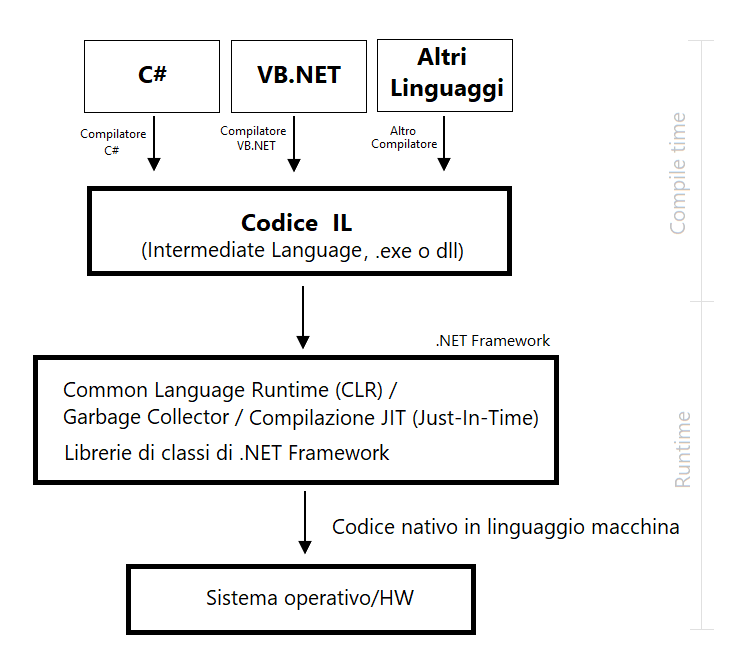
\includegraphics[scale = 0.6]{Immagini/architettura-framework-dotnet.png}
    \caption{Architettura della piattaforma .NET Framework}
    \label{fig:my_label}
\end{figure}
\hspace{-0.6cm}Nella \textbf{Figura 3.9} sono illustrate le relazioni, in fase di compilazione (\textit{Compile Time}) e di esecuzione (\textit{Runtime}), tra i file di codice sorgente C\#, o degli altri linguaggi, le librerie di classi di \textit{.NET Framework}, gli \textit{assembly} e il CLR.
\\Il codice sorgente scritto in C\# viene compilato in un linguaggio intermedio (\textit{Intermediate Language}, IL). Il codice IL viene archiviato sul disco in un file eseguibile denominato \textit{assembly}, in genere con estensione EXE o DLL.
\\Quando viene eseguito il programma C\#, l'\textit{assembly} viene caricato nel CLR, e se i requisiti di sicurezza sono soddisfatti, il CLR esegue una compilazione \textit{Just-In-Time} (JIT) per convertire il codice IL in istruzioni del linguaggio macchina nativo.
\\Le librerie di classi sono una raccolta completa e orientata agli oggetti di tipi riusabili, da utlizzare per lo sviluppo di applicazioni, da quelle tradizionali a riga di comando o con interfaccia utente grafica (GUI, \textit{Graphical User Interface}) a quelle basate sulle più recenti innovazioni offerte da ASP.NET, quali Web Form e servizi Web XML, Web API e tanto altro.
\begin{lstlisting}[caption = Esempio di utilizzo di librerie in C\#]
using System.Collections;
using System.Collections.Generic;
using UnityEngine;
...
\end{lstlisting}
\subsection{MonoBehaviour}
\textit{MonoBehaviour}\cite{Mono} è la classe di base che tutti gli script in \textit{Unity} devono avere.\\La classe MonoBehaviour espone una serie di funzioni evento che vengono chiamate da \textit{Unity} al verificarsi di determinate condizioni.\\
Ad esempio, un evento come \textit{MonoBehaviour.OnCollisionEnter()} si verificherà ogni volta che un oggetto entra in collisione con un altro oggetto.
\\Quando questo accade, \textit{Unity} provvederà a richiamare automaticamente il metodo \textit{OnCollisionEnter}(la lista degli eventi è consultabile qui\cite{Eventi}).
\\Le funzioni evento vanno richiamate all'interno di metodi specifici della classe MonoBehaviour, i 3 principali sono:
\begin{itemize}
    \item \textit{Awake}();
    \item \textit{Start}();
    \item \textit{Update}().
\end{itemize}
I Metodi \textit{\textit{Awake}} e \textit{\textit{Start}} vengono chiamati una sola volta nel ciclo di vita di un oggetto. 
\\La differenza fra i due sta nel fatto che \textit{\textit{Awake}} viene chiamato molto presto, durante la preparazione della scena. In quel momento gli oggetti in scena non sono completamente valorizzati, quindi in \textit{Awake} è sconsigliato svolgere operazioni che richiedono i valori di altri oggetti, come ad esempio leggere il \textit{tag} di un altro oggetto in scena.
\\\textit{\textit{Start}} è utile per eseguire operazioni di preparazione al gioco, come la ricerca di elementi nella scena di cui vogliamo salvare un riferimento per poi lavorarci più avanti durante l'esecuzione.
\\Molto interessante è il tempismo di chiamata dei due metodi a seconda dello stato, attivo o disattivo, dello script in cui compaiono \textit{Awake} e \textit{Start} e il \textit{GameObject} su cui risiede lo script, che viene illustrato nella seguente immagine:
\begin{figure}[H]
    \centering
    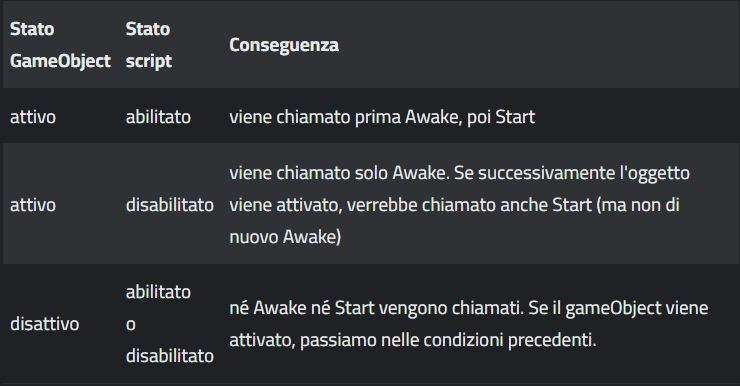
\includegraphics[scale = 0.6]{Immagini/Awake}.jpg]
    \caption{Tempismo di chiamata dei metodi \textit{Awake} e \textit{Start}}
    \label{fig:my_label}
\end{figure} 
\hspace{-0.6cm}Il metodo \textit{Update}, invece, viene chiamato ad ogni frame, il che lo rende molto utile, per esempio, per eseguire azioni come aggiornare o modificare la posizione di oggetti nella scena, per tenere traccia dell'input del giocatore e attribuire comportamenti periodici agli oggetti.
\begin{lstlisting}[language = {[Sharp]C}, caption = {Esempio di utilizzo dei metodi Start e Update}, label{Script}]
using UnityEngine;
using System.Collections;

public class GameObject: MonoBehaviour {

void Start(){ . . . }

void Update(){ . . . }
} 
\end{lstlisting}
\subsection{Librerie Utilizzate}
L'utilizzo di librerie è essenziale per la progettazione e sviluppo di software, sono estremamente utili perché forniscono una collezione di entità di base pronte per l'uso, evitando al programmatore di dover riscrivere ogni volta le stesse funzioni o strutture dati e facilitando così le operazioni di sviluppo e manutenzione.
\\Per la realizzazione di questo prototipo si distinguono in due tipologie di librerie:
\begin{itemize}
    \item Le librerie interne presenti nello \textit{\gls{Unity Registry}};
    \item Le librerie \textit{Photon} importate dall'\textit{\gls{Asset Store}}.
\end{itemize}
\subsubsection{Librerie Interne}
Le principali librerie Interne utilizzate sono:
\begin{itemize}
    \item UnityEngine, raccoglie le classi fondamentali e di riferimento per ogni progetto \textit{Unity}: 
    \begin{itemize}
    \item UnityEngine.Events\cite{UnityEvents};
    \item UnityEngine.InputSystem\cite{UnityInputSystem};
    \item UnityEngine.XR.Interaction.Toolkit\cite{XRToolkit};
    \item UnityEngine.UI\cite{UI}.
    \end{itemize}
    \item{System}, contiene le classi fondamentali e di base che definiscono eventi, gestori di eventi, interfacce, attributi, eccezioni di elaborazione e tipi di dati di riferimento e valore usati comunemente:
    \begin{itemize}
    \item System.Collections\cite{Collection};
    \item System.Collections.Generic\cite{CollectionGeneric}.
    \end{itemize}
    \item TMPro\cite{TMP_pro}, offre soluzioni per il testo relativo all'interfaccia utente dell'applicazione finale.
\end{itemize}
\subsubsection{Librerie Photon}
Le librerie \textit{Photon} importate sono:
\begin{itemize}
    \item Photon.PUN\cite{Photon_PUN};
    \item Photon.Chat\cite{Photon_Chat};
    \item Photon.Voice\cite{Photon_Voice}.
\end{itemize}
\section{Photon Engine}
\begin{figure}[H]
    \centering
    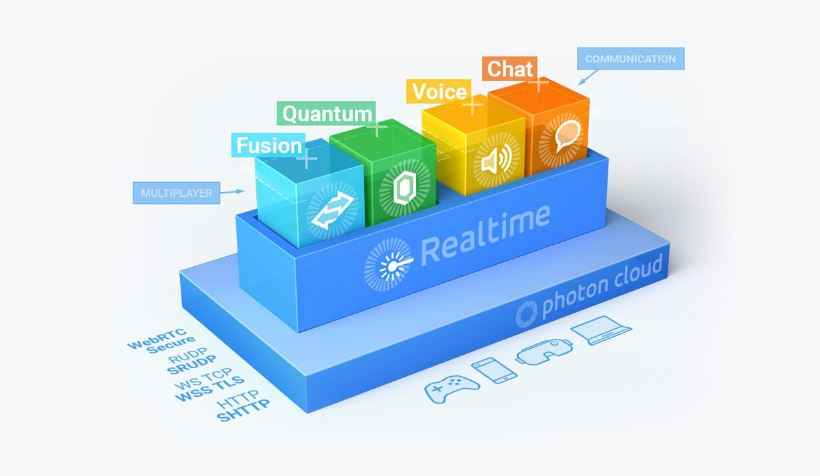
\includegraphics[scale = 0.7]{Immagini/PhotonStructure.jpg}
    \caption{Struttura di Photon engine}
    \label{fig:my_label}
\end{figure}
\textit{Photon Engine\cite{Photon}} è un motore grafico specializzato nello sviluppo di applicazioni multi-utente.
Nella \textbf{Figura 3.11} si può vedere che il motore grafico è composto da due parti principali:
\begin{itemize}
    \item \textit{Photon Cloud};
    \item \textit{Photon Realtime}.
\end{itemize}
Il \textit{Photon Cloud} è un soluzione \textbf{SaaS} (\textit{Software As A Service}), questo significa che il \textit{\gls{runtime}} locale sul dispositivo client ha già riferimenti al sistema server, che è rilasciato e gestito in un ambiente cloud esterno. \\Il sistema, perciò, non è completamente sotto controllo dell'utente, ma ha dipendenze da componenti remoti di \textit{Photon}.
\\Questo è il motivo principale per cui i servizi offerti da \textit{Photon} sono stati scelti per sviluppare le funzionalità di rete.
\\Il \textit{Photon Realtime} è la parte del motore grafico composta dai \textit{packages} e dalle librerie, quindi sono gli strumenti che l'utente deve utilizzare per sviluppare la propria applicazione multi-utente.
\\In particolare per lo sviluppo del prototipo sono state utilizzate 3 applicazioni del \textit{Photon Realtime}:
\begin{itemize}
    \item PUN (\textit{Photon Unity Networking}), utilizzata per la connessione tra utenti;
    \item \textit{Photon Voice}, utilizzata per la comunicazione vocale tra utenti;
    \item \textit{Photon Chat}, utlizzata per la comunicazione via chat tra utenti.
\end{itemize}
\subsection{Implementazione di PUN in Unity}
In questa sezione saranno illustrati i passaggi fondamentali per la preparazione di un progetto \textit{Unity} alle funzionalità multi-utente di \textit{Photon}.
\begin{figure}[H]
    \centering
    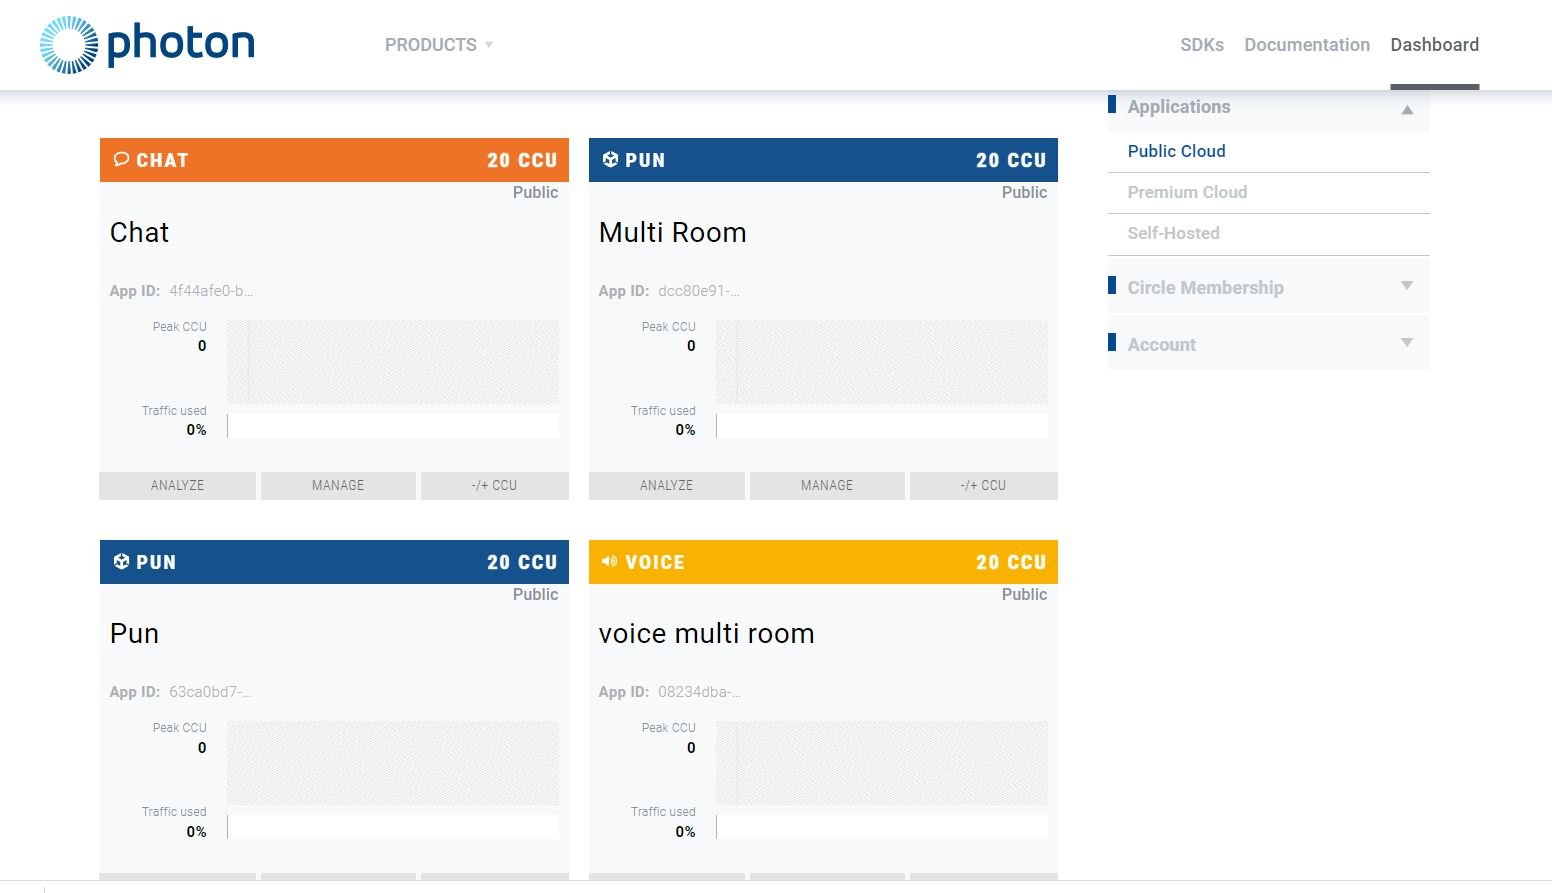
\includegraphics[scale = 0.3]{Immagini/Sitophoton.jpg}
    \caption{Dashboard delle applicazioni Photon Realtime}
    \label{fig:my_label}
\end{figure}
\hspace{-0.6cm}La \textbf{Figura 3.12} mostra la dashboard delle applicazioni \textit{Photon} Realtime descritte in precedenza, l'accesso alla dashboard è consentito dopo aver creato un account \textit{Photon} gratuitamente.
\\Ogni applicazione, Chat, PUN o Voice, è caratterizzata da un App ID che, dopo aver installato il package PUN
dall'Asset Store di \textit{Unity}, va inserito nell'apposito campo nella sezione dell'editor \textit{`Window/Photon Unity Networking/Highlight Server Setting`}.
\begin{figure}[H]
    \centering
    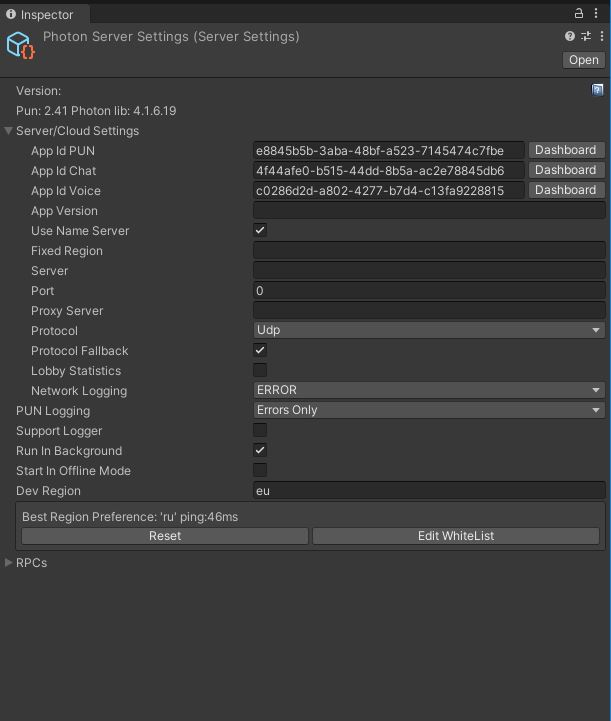
\includegraphics[scale = 0.7]{Immagini/Setting.jpg}
    \caption{Photon Server Settings}
    \label{fig:my_label}
\end{figure}
\hspace{-0.6cm}A questo punto la fase di preparazione del progetto alle funzionalità network è terminata e si può procedere con la progettazione delle funzioni per la connettività tra utenti.